\documentclass{article}
\usepackage{mathtools}
\usepackage[top=2in, bottom=1.5in, left=1in, right=1in]{geometry}
\usepackage{graphicx}
\usepackage[normalem]{ulem}
\usepackage{fancyhdr}
\pagestyle{fancyplain}


\rhead{A. Shawn Bandy 
(003635396)}

\begin{document}
\title{Homework \#3}
\author{A. Shawn Bandy}
\date{February 17, 2013}
\maketitle
\begin{enumerate}
\item[Q1.] Suppose you are interested in estimating the effect of hours spent in an SAT preparation course (hours) on the total SAT score (sat). The population is all college-bound high school seniors graduating in a particular year.
\begin{enumerate}
\item[a.]Suppose you are given a grant to run a controlled experiment. Explain how you would structure the experiment in order to estimate the causal effect of hours on sat. 
\newline\newline
For each subject, I would assign a number of hours to study determined by randomly selecting values from a normal distribution with the the estimated sample mean and standard deviation.  Then I would collect the SAT scores for each student.
\newline
\item[b.]Consider the more realistic case where students choose the number of hours they spend on SAT preparation and whether or not to take an SAT-prep course. In this case, you can only randomly select sat and hours from the population of students.  The population model is: $sat = \beta_0 + \beta_1 * hours + u$ where, because of the intercept, E(u) =0. List one factor that might explain sat that is likely included in u. Do you think this factor is correlated with hours? If this factor were correlated with hours, why might that be a problem? 
\newline\newline
One factor that might be included in u is high school GPA: a higher GPA probably covaries with {\it{sat}}.  I do believe GPA would be correlated with {\it{hours}} and if so, it would suggest that $E(u) \neq 0$
\newline
\item[c.]In the equation from part (ii), what should the sign of $\beta_1$ be if the preparation course is effective?
\newline\newline
The sign for $\beta_1$ should be positive if the preparation course is effective.
\newline
\end{enumerate}
\newpage
\item[Q2.] Use the results from L1 to calculate the following. Even though the regression output tells you the answers, show how they are calculated assuming you had the other output but you did not have the regression results. Please show what formula you used and the steps you used to get to the final answer. You can always use the output to see if you did it right!
\linebreak
\begin{enumerate}
\item[a.] The coefficient for beauty, using the formula. (Hint: What is the numerator? What is the denominator?)
\newline\newline
$\hat\beta_1 = \frac{cov(x,y)}{var(x)}= \frac{0.082722}{0.621965} = 0.133001$
\newline
\item[b.] Write down the null and alternative hypotheses to test if the coefficient on beauty is equal to zero. 
\newline\newline
${H}_0: \hat\beta_1 \neq 0$
\newline
${H}_0: \hat\beta_1 = 0$
\newline
I would reject the null hypothesis at the 95\% confidence level.
\newline
\item[c.] Calculate the t-statistic to test the null hypothesis from part b). Note: In this part it is OK to use the standard error calculated by the regression output rather than having to calculate it. 
\newline\newline
$t = \frac{B_1}{S_{B_1}} = \frac{0.133001}{0.0321775} = 4.13335$
\newline
\item[d.]To test the hypothesis in part b) with a confidence level of 95% level, then the critical t-value is 1.96. Would you reject or accept (fail to reject) the null hypothesis? Explain. 
\newline\newline
$|4.13335| > (t-critical = 1.96)$
\newline
\item[e.] Calculate the R2 for this model. What does it represent? 
\newline\newline
$R^2 = 1 - \frac{RSS}{TSS} = 1 - \frac{137.155613}{142.23862} = 0.035736$
\newline\newline
$R^2$ is the amount of variation that is explained by the regression model: in this case about 3 percent.
\item[f.]Compare your results to a), c) and e) to the output from your regression in L1. Are they the same? 
\newline\newline
Yes, the are the same.
\end{enumerate}
\newpage
\item[L1.]
{\tiny
\begin{verbatim}
--------------------------------------------------------------------------------
      name:  <unnamed>
       log:  C:\Users\cla-spa206.CAMPUS-DOMAIN\Downloads\lab3\lab3\teaching.log
  log type:  text
 opened on:  14 Feb 2013, 11:13:18

. /*a. Create a graph that includes both a scatter plot of average course evalua
> tion (course_eval) vs. instructor’s beauty
>  (beauty) and the fitted line. Save this scatter plot as scattereval_beauty.em
> f so it can be printed and turned in with
>  your assignment.*/
> 
>  twoway (lfit course_eval beauty)(scatter course_eval beauty);

.  graph export scattereval_beauty.emf, replace;
(file C:\Users\cla-spa206.CAMPUS-DOMAIN\Downloads\lab3\lab3\scattereval_beauty.e
> mf written in Enhanced Metafile format)

.  graph export scattereval_beauty.png, replace;
(file scattereval_beauty.png written in PNG format)

.  //Note: this is for my use:  .emf is difficult to work with on Mac/Linux
>  
> /*b. Using the scatter plot and the fitted line from a), does it appear that c
> ourse evaluations and beauty are related?
>  Explain why.
>  //TODO Interpretation
>  
>  */
> 
> 
>  
> /*c. Use the summarize command to look at the description of the variables in 
> this dataset.*/
> 
> summarize;

    Variable |       Obs        Mean    Std. Dev.       Min        Max
-------------+--------------------------------------------------------
    minority |       463    .1382289    .3455134          0          1
         age |       463    48.36501    9.802742         29         73
      female |       463    .4211663    .4942802          0          1
   onecredit |       463    .0583153    .2345922          0          1
      beauty |       463    4.75e-08    .7886477  -1.450494   1.970023
-------------+--------------------------------------------------------
 course_eval |       463    3.998272    .5548656        2.1          5
       intro |       463    .3390929    .4739135          0          1
   nnenglish |       463    .0604752    .2386229          0          1

. /*d. Use the covariance option for the correlate command to get the covariance
>  between course_eval and beauty.*/
> 
> correlate course_eval beauty, covariance;
(obs=463)

             | course~l   beauty
-------------+------------------
 course_eval |  .307876
      beauty |  .082722  .621965


. /*e. Use the regression command to estimate the following linear regression mo
> del
> CourseEvaluations_i = Beta_zero * Beauty + u_i*/
> 
> regress course_eval beauty;

      Source |       SS       df       MS              Number of obs =     463
-------------+------------------------------           F(  1,   461) =   17.08
       Model |  5.08300731     1  5.08300731           Prob > F      =  0.0000
    Residual |  137.155613   461  .297517598           R-squared     =  0.0357
-------------+------------------------------           Adj R-squared =  0.0336
       Total |   142.23862   462  .307875801           Root MSE      =  .54545

------------------------------------------------------------------------------
 course_eval |      Coef.   Std. Err.      t    P>|t|     [95% Conf. Interval]
-------------+----------------------------------------------------------------
      beauty |   .1330014   .0321775     4.13   0.000     .0697687    .1962342
       _cons |   3.998272   .0253493   157.73   0.000     3.948458    4.048087
------------------------------------------------------------------------------
. /*f. What is the interpretation of the intercept term0ßin this regression mode
> l.
> //TODO Interpretation*/
> 
> 
> /*g. Using the regression output, what is the value of the estimated intercept
>  0ˆß?
> //TODO Interpretation*/
> 
> 
> /*h. What is the interpretation of the slope term1ßin this regression model. 
> //TODO Interpretation*/
> 
> 
> /*i. Using the regression output, what is the value of the estimated slope 1ˆß
> ?
> Is it significantly different from zero? How do you know?
> //TODO Interpretaion*/
> 
> 
> /*j. Suppose Professor Smith is of average beauty, while Professor Miller is o
> ne standard deviation above the average beauty.
>  Using the regression output and the summary statistics, predict Professor Smi
> th’s and Professor Miller’s course evaluations.
>  //TODO Interpretaion*/
> 
> /*k. Does this model explain a large fraction of the variance in course evalua
> tions 
> //TODO Interpretaion*/
> 
> log close;
      name:  <unnamed>
       log:  C:\Users\cla-spa206.CAMPUS-DOMAIN\Downloads\lab3\lab3\teaching.log
  log type:  text
 closed on:  14 Feb 2013, 11:13:19
--------------------------------------------------------------------------------

/* 	A. Shawn Bandy
	Lab #3 
	February 12th, 2013
*/
/* close previous run do-files */
cap log close
set more 1
clear
#delimit ;

cd "C:\Users\cla-spa206.CAMPUS-DOMAIN\Downloads\lab3\lab3";

use "TeachingRatings";
log using teaching.log , replace;

/*a. Create a graph that includes both a scatter plot of average course evaluation (course_eval) vs. instructor’s beauty
 (beauty) and the fitted line. Save this scatter plot as scattereval_beauty.emf so it can be printed and turned in with
 your assignment.*/

 twoway (lfit course_eval beauty)(scatter course_eval beauty);
 graph export scattereval_beauty.emf, replace;
 graph export scattereval_beauty.png, replace; //Note: this is for my use:  .emf is difficult to work with on Mac/Linux
 
/*b. Using the scatter plot and the fitted line from a), does it appear that course evaluations and beauty are related?
 Explain why.
 //TODO Interpretation
 
 */
 
/*c. Use the summarize command to look at the description of the variables in this dataset.*/

summarize;

/*d. Use the covariance option for the correlate command to get the covariance between course_eval and beauty.*/

correlate course_eval beauty, covariance;

/*e. Use the regression command to estimate the following linear regression model
CourseEvaluations_i = Beta_zero * Beauty + u_i*/

regress course_eval beauty;
/*f. What is the interpretation of the intercept term0ßin this regression model.
//TODO Interpretation*/


/*g. Using the regression output, what is the value of the estimated intercept 0ˆß?
//TODO Interpretation*/


/*h. What is the interpretation of the slope term1ßin this regression model. 
//TODO Interpretation*/


/*i. Using the regression output, what is the value of the estimated slope 1ˆß?
Is it significantly different from zero? How do you know?
//TODO Interpretaion*/


/*j. Suppose Professor Smith is of average beauty, while Professor Miller is one standard deviation above the average beauty.
 Using the regression output and the summary statistics, predict Professor Smith’s and Professor Miller’s course evaluations.
 //TODO Interpretaion*/

/*k. Does this model explain a large fraction of the variance in course evaluations 
//TODO Interpretaion*/

log close;

\end{verbatim}
}
\newpage
\item[L1 Interpretation] The questions below are part of the L1 procedure.
\begin{enumerate}
\item[b.] Using the scatter plot and the fitted line from a), does it appear that course evaluations and beauty are related? Explain why.
\newline\newline
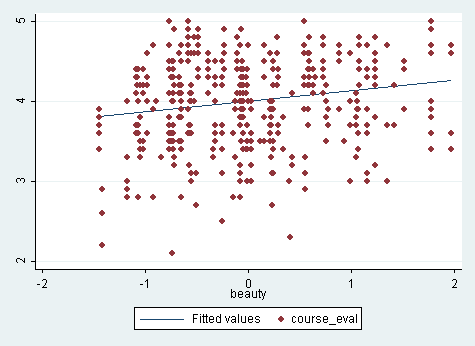
\includegraphics{scattereval_beauty}
\newline\newline
{Although I cannot say that there is no relationship at all, I do not see any linear relation in this scatter plot.  If there were a linear relation, I would expect to see the {\it{course\_eval}} plots near the fitted line.  In this case the plots are truly scattered over the area of the graph.}
\item[f.] What is the interpretation of the intercept term $\beta_0$ in this regression model.
\newline\newline
$\beta_0$ is the expected value for {\it{course\_eval}} when {\it{beauty}} equals zero.  
\item[g.]Using the regression output, what is the value of the estimated intercept $\beta_0$?
\newline\newline
According to the regression output, $\beta_0$ equals 3.998272.
\newline
\item[h.] What is the interpretation of the slope term $\beta_1$ in this regression model? 
\newline\newline
For each unit change in {\it{beauty}}, {\it{course\_eval}} changes by 0.1330014 units.
\newline
\item[i.] Using the regression output, what is the value of the estimated slope $\beta_1$ ?  Is it significantly different from zero? How do you know?
\newline\newline
The value of the estimated slope of $\beta_1$ is 0.1330014 and is significantly different than zero at the 95\% confidence level because 0 is between 3.948458 and 4.048087.
\newline
\item[j.] Suppose Professor Smith is of average beauty, while Professor Miller is one standard deviation above the average beauty.  Using the regression output and the summary statistics, predict Professor Smith\'’s and Professor Miller\'’s course evaluations.
\newline\newline
\uline{Professor Smith}\newline
$3.998272 + 0.1330014 * (4.85 * 10^{-8}) = 3.99827$
\newline\newline
\uline{Professor Miller}\newline
$3.998272 + 0.1330014 * (4.85 * 10^{-8} + 0.7886477) = 4.10316$
\newline
\item[k.]Does this model explain a large fraction of the variance in course evaluations?
\newline\newline
No.  $\bar{R^2} = 0.0336$ or about 3\% of the variation in {\it{course\_eval}} is explained by this regression model.
\end{enumerate}
\end{enumerate}
\end{document}